% Options for packages loaded elsewhere
\PassOptionsToPackage{unicode}{hyperref}
\PassOptionsToPackage{hyphens}{url}
\PassOptionsToPackage{dvipsnames,svgnames,x11names}{xcolor}
%
\documentclass[
  letterpaper,
  DIV=11,
  numbers=noendperiod]{scrreprt}

\usepackage{amsmath,amssymb}
\usepackage{iftex}
\ifPDFTeX
  \usepackage[T1]{fontenc}
  \usepackage[utf8]{inputenc}
  \usepackage{textcomp} % provide euro and other symbols
\else % if luatex or xetex
  \usepackage{unicode-math}
  \defaultfontfeatures{Scale=MatchLowercase}
  \defaultfontfeatures[\rmfamily]{Ligatures=TeX,Scale=1}
\fi
\usepackage{lmodern}
\ifPDFTeX\else  
    % xetex/luatex font selection
\fi
% Use upquote if available, for straight quotes in verbatim environments
\IfFileExists{upquote.sty}{\usepackage{upquote}}{}
\IfFileExists{microtype.sty}{% use microtype if available
  \usepackage[]{microtype}
  \UseMicrotypeSet[protrusion]{basicmath} % disable protrusion for tt fonts
}{}
\makeatletter
\@ifundefined{KOMAClassName}{% if non-KOMA class
  \IfFileExists{parskip.sty}{%
    \usepackage{parskip}
  }{% else
    \setlength{\parindent}{0pt}
    \setlength{\parskip}{6pt plus 2pt minus 1pt}}
}{% if KOMA class
  \KOMAoptions{parskip=half}}
\makeatother
\usepackage{xcolor}
\setlength{\emergencystretch}{3em} % prevent overfull lines
\setcounter{secnumdepth}{5}
% Make \paragraph and \subparagraph free-standing
\ifx\paragraph\undefined\else
  \let\oldparagraph\paragraph
  \renewcommand{\paragraph}[1]{\oldparagraph{#1}\mbox{}}
\fi
\ifx\subparagraph\undefined\else
  \let\oldsubparagraph\subparagraph
  \renewcommand{\subparagraph}[1]{\oldsubparagraph{#1}\mbox{}}
\fi

\usepackage{color}
\usepackage{fancyvrb}
\newcommand{\VerbBar}{|}
\newcommand{\VERB}{\Verb[commandchars=\\\{\}]}
\DefineVerbatimEnvironment{Highlighting}{Verbatim}{commandchars=\\\{\}}
% Add ',fontsize=\small' for more characters per line
\usepackage{framed}
\definecolor{shadecolor}{RGB}{241,243,245}
\newenvironment{Shaded}{\begin{snugshade}}{\end{snugshade}}
\newcommand{\AlertTok}[1]{\textcolor[rgb]{0.68,0.00,0.00}{#1}}
\newcommand{\AnnotationTok}[1]{\textcolor[rgb]{0.37,0.37,0.37}{#1}}
\newcommand{\AttributeTok}[1]{\textcolor[rgb]{0.40,0.45,0.13}{#1}}
\newcommand{\BaseNTok}[1]{\textcolor[rgb]{0.68,0.00,0.00}{#1}}
\newcommand{\BuiltInTok}[1]{\textcolor[rgb]{0.00,0.23,0.31}{#1}}
\newcommand{\CharTok}[1]{\textcolor[rgb]{0.13,0.47,0.30}{#1}}
\newcommand{\CommentTok}[1]{\textcolor[rgb]{0.37,0.37,0.37}{#1}}
\newcommand{\CommentVarTok}[1]{\textcolor[rgb]{0.37,0.37,0.37}{\textit{#1}}}
\newcommand{\ConstantTok}[1]{\textcolor[rgb]{0.56,0.35,0.01}{#1}}
\newcommand{\ControlFlowTok}[1]{\textcolor[rgb]{0.00,0.23,0.31}{#1}}
\newcommand{\DataTypeTok}[1]{\textcolor[rgb]{0.68,0.00,0.00}{#1}}
\newcommand{\DecValTok}[1]{\textcolor[rgb]{0.68,0.00,0.00}{#1}}
\newcommand{\DocumentationTok}[1]{\textcolor[rgb]{0.37,0.37,0.37}{\textit{#1}}}
\newcommand{\ErrorTok}[1]{\textcolor[rgb]{0.68,0.00,0.00}{#1}}
\newcommand{\ExtensionTok}[1]{\textcolor[rgb]{0.00,0.23,0.31}{#1}}
\newcommand{\FloatTok}[1]{\textcolor[rgb]{0.68,0.00,0.00}{#1}}
\newcommand{\FunctionTok}[1]{\textcolor[rgb]{0.28,0.35,0.67}{#1}}
\newcommand{\ImportTok}[1]{\textcolor[rgb]{0.00,0.46,0.62}{#1}}
\newcommand{\InformationTok}[1]{\textcolor[rgb]{0.37,0.37,0.37}{#1}}
\newcommand{\KeywordTok}[1]{\textcolor[rgb]{0.00,0.23,0.31}{#1}}
\newcommand{\NormalTok}[1]{\textcolor[rgb]{0.00,0.23,0.31}{#1}}
\newcommand{\OperatorTok}[1]{\textcolor[rgb]{0.37,0.37,0.37}{#1}}
\newcommand{\OtherTok}[1]{\textcolor[rgb]{0.00,0.23,0.31}{#1}}
\newcommand{\PreprocessorTok}[1]{\textcolor[rgb]{0.68,0.00,0.00}{#1}}
\newcommand{\RegionMarkerTok}[1]{\textcolor[rgb]{0.00,0.23,0.31}{#1}}
\newcommand{\SpecialCharTok}[1]{\textcolor[rgb]{0.37,0.37,0.37}{#1}}
\newcommand{\SpecialStringTok}[1]{\textcolor[rgb]{0.13,0.47,0.30}{#1}}
\newcommand{\StringTok}[1]{\textcolor[rgb]{0.13,0.47,0.30}{#1}}
\newcommand{\VariableTok}[1]{\textcolor[rgb]{0.07,0.07,0.07}{#1}}
\newcommand{\VerbatimStringTok}[1]{\textcolor[rgb]{0.13,0.47,0.30}{#1}}
\newcommand{\WarningTok}[1]{\textcolor[rgb]{0.37,0.37,0.37}{\textit{#1}}}

\providecommand{\tightlist}{%
  \setlength{\itemsep}{0pt}\setlength{\parskip}{0pt}}\usepackage{longtable,booktabs,array}
\usepackage{calc} % for calculating minipage widths
% Correct order of tables after \paragraph or \subparagraph
\usepackage{etoolbox}
\makeatletter
\patchcmd\longtable{\par}{\if@noskipsec\mbox{}\fi\par}{}{}
\makeatother
% Allow footnotes in longtable head/foot
\IfFileExists{footnotehyper.sty}{\usepackage{footnotehyper}}{\usepackage{footnote}}
\makesavenoteenv{longtable}
\usepackage{graphicx}
\makeatletter
\def\maxwidth{\ifdim\Gin@nat@width>\linewidth\linewidth\else\Gin@nat@width\fi}
\def\maxheight{\ifdim\Gin@nat@height>\textheight\textheight\else\Gin@nat@height\fi}
\makeatother
% Scale images if necessary, so that they will not overflow the page
% margins by default, and it is still possible to overwrite the defaults
% using explicit options in \includegraphics[width, height, ...]{}
\setkeys{Gin}{width=\maxwidth,height=\maxheight,keepaspectratio}
% Set default figure placement to htbp
\makeatletter
\def\fps@figure{htbp}
\makeatother
\newlength{\cslhangindent}
\setlength{\cslhangindent}{1.5em}
\newlength{\csllabelwidth}
\setlength{\csllabelwidth}{3em}
\newlength{\cslentryspacingunit} % times entry-spacing
\setlength{\cslentryspacingunit}{\parskip}
\newenvironment{CSLReferences}[2] % #1 hanging-ident, #2 entry spacing
 {% don't indent paragraphs
  \setlength{\parindent}{0pt}
  % turn on hanging indent if param 1 is 1
  \ifodd #1
  \let\oldpar\par
  \def\par{\hangindent=\cslhangindent\oldpar}
  \fi
  % set entry spacing
  \setlength{\parskip}{#2\cslentryspacingunit}
 }%
 {}
\usepackage{calc}
\newcommand{\CSLBlock}[1]{#1\hfill\break}
\newcommand{\CSLLeftMargin}[1]{\parbox[t]{\csllabelwidth}{#1}}
\newcommand{\CSLRightInline}[1]{\parbox[t]{\linewidth - \csllabelwidth}{#1}\break}
\newcommand{\CSLIndent}[1]{\hspace{\cslhangindent}#1}

\usepackage{fontspec}
\usepackage{multirow}
\usepackage{multicol}
\usepackage{colortbl}
\usepackage{hhline}
\newlength\Oldarrayrulewidth
\newlength\Oldtabcolsep
\usepackage{longtable}
\usepackage{array}
\usepackage{hyperref}
\usepackage{float}
\usepackage{wrapfig}
\KOMAoption{captions}{tableheading}
\makeatletter
\makeatother
\makeatletter
\@ifpackageloaded{bookmark}{}{\usepackage{bookmark}}
\makeatother
\makeatletter
\@ifpackageloaded{caption}{}{\usepackage{caption}}
\AtBeginDocument{%
\ifdefined\contentsname
  \renewcommand*\contentsname{Tabla de contenidos}
\else
  \newcommand\contentsname{Tabla de contenidos}
\fi
\ifdefined\listfigurename
  \renewcommand*\listfigurename{Listado de Figuras}
\else
  \newcommand\listfigurename{Listado de Figuras}
\fi
\ifdefined\listtablename
  \renewcommand*\listtablename{Listado de Tablas}
\else
  \newcommand\listtablename{Listado de Tablas}
\fi
\ifdefined\figurename
  \renewcommand*\figurename{Figura}
\else
  \newcommand\figurename{Figura}
\fi
\ifdefined\tablename
  \renewcommand*\tablename{Tabla}
\else
  \newcommand\tablename{Tabla}
\fi
}
\@ifpackageloaded{float}{}{\usepackage{float}}
\floatstyle{ruled}
\@ifundefined{c@chapter}{\newfloat{codelisting}{h}{lop}}{\newfloat{codelisting}{h}{lop}[chapter]}
\floatname{codelisting}{Listado}
\newcommand*\listoflistings{\listof{codelisting}{Listado de Listados}}
\makeatother
\makeatletter
\@ifpackageloaded{caption}{}{\usepackage{caption}}
\@ifpackageloaded{subcaption}{}{\usepackage{subcaption}}
\makeatother
\makeatletter
\@ifpackageloaded{tcolorbox}{}{\usepackage[skins,breakable]{tcolorbox}}
\makeatother
\makeatletter
\@ifundefined{shadecolor}{\definecolor{shadecolor}{rgb}{.97, .97, .97}}
\makeatother
\makeatletter
\makeatother
\makeatletter
\makeatother
\ifLuaTeX
\usepackage[bidi=basic]{babel}
\else
\usepackage[bidi=default]{babel}
\fi
\babelprovide[main,import]{spanish}
% get rid of language-specific shorthands (see #6817):
\let\LanguageShortHands\languageshorthands
\def\languageshorthands#1{}
\ifLuaTeX
  \usepackage{selnolig}  % disable illegal ligatures
\fi
\IfFileExists{bookmark.sty}{\usepackage{bookmark}}{\usepackage{hyperref}}
\IfFileExists{xurl.sty}{\usepackage{xurl}}{} % add URL line breaks if available
\urlstyle{same} % disable monospaced font for URLs
\hypersetup{
  pdftitle={Estimación de la integridad ecosistémica de las costas arenosas mexicanas a través de técnicas de aprendizaje de máquina},
  pdfauthor={Octavio Pérez-Maqueo; Miguel Equihua},
  pdflang={es},
  colorlinks=true,
  linkcolor={blue},
  filecolor={Maroon},
  citecolor={Blue},
  urlcolor={Blue},
  pdfcreator={LaTeX via pandoc}}

\title{Estimación de la integridad ecosistémica de las costas arenosas
mexicanas a través de técnicas de aprendizaje de máquina}
\usepackage{etoolbox}
\makeatletter
\providecommand{\subtitle}[1]{% add subtitle to \maketitle
  \apptocmd{\@title}{\par {\large #1 \par}}{}{}
}
\makeatother
\subtitle{Proyecto Conahcyt de ciencia de frontera (CF-2023-G-1497)}
\author{Octavio Pérez-Maqueo \and Miguel Equihua}
\date{2024-05-23}

\begin{document}
\maketitle
\ifdefined\Shaded\renewenvironment{Shaded}{\begin{tcolorbox}[boxrule=0pt, borderline west={3pt}{0pt}{shadecolor}, frame hidden, sharp corners, interior hidden, enhanced, breakable]}{\end{tcolorbox}}\fi

\renewcommand*\contentsname{Tabla de contenidos}
{
\hypersetup{linkcolor=}
\setcounter{tocdepth}{2}
\tableofcontents
}
\bookmarksetup{startatroot}

\hypertarget{preface}{%
\chapter*{Preface}\label{preface}}
\addcontentsline{toc}{chapter}{Preface}

\markboth{Preface}{Preface}

Este es el documento de registro de avances del proyecto
\textbf{Estimación de la integridad ecosistémica de las costas arenosas
mexicanas a través de técnicas de aprendizaje de máquina}

\bookmarksetup{startatroot}

\hypertarget{resumen}{%
\chapter{Resumen}\label{resumen}}

México, como otros países, inició la implementación de un sistema de
cuentas de ecosistemas cuyo propósito es calcular y poner regularmente a
disposición de la sociedad información sobre la extensión y la condición
de los ecosistemas, así como de la capacidad para obtener los diversos
beneficios que la naturaleza provee como servicios ecosistémicos. Como
parte de un piloto mundial, México desarrolló un sistema de contabilidad
para ecosistemas terrestres (INEGI 2021). Ahora, hay el interés en
extender el sistema para incluir los ambientes costeros, marinos y
acuáticos continentales. Para los ecosistemas terrestres México
desarrolló una propuesta que aprovecha datos masivos (Big data) y la
aplicación de técnicas de inteligencia artificial (IA). La experiencia
mostró que este planteamiento puede ser de enorme ayuda para llevar a
cabo una contabilidad de ecosistemas a gran escala. Las técnicas de IA
son atípicas dentro del ámbito de la contabilidad ambiental y por tanto
se estima que la estrategia iniciada en nuestro país es innovadora.
Además, las nuevas propuestas en el uso de las técnicas de aprendizaje
de máquina apuntan a preferir formulaciones causales que si bien son
procesadas por máquinas, produzcan resultados entendibles para los
usuarios humanos. Esto es lo que está emergiendo como ``Inteligencia
artificial interpretable'' (IAI por las siglas en inglés, Mihaljevic et
al 2021). Una aproximación del tipo IAI para el caso de las cuentas de
ecosistemas permitiría, con base en datos y un enfoque sistémico, un
mayor entendimiento de las relaciones entre las acciones de origen
antrópico y su repercusión en los ecosistemas del país y en los
servicios que estos proporcionan. En este proyecto, se propone evaluar
como prueba de concepto, la condición de las costas arenosas (playas y
dunas) de todo el país, por medio del cálculo de un índice de integridad
de los ecosistemas de costas arenosas (IIECA) bajo el paradigma de IAI.

\bookmarksetup{startatroot}

\hypertarget{introducciuxf3n}{%
\chapter{Introducción}\label{introducciuxf3n}}

El proyecto \textbf{Estimación de la integridad ecosistémica de las
costas arenosas mexicanas a través de técnicas de aprendizaje de
máquina} se propone generar estimaciones de la condición en la que se
encuentran los ecosistemas costeros, especialmente los arenosos, del
país con una representación raster y resolución geográfica de pixeles de
3 segundos (aproximadamente 100 m). También se está considerando tener
una valoración de mayor resolución para la zona costera de Quintana Roo,
en donde se propone lograr una resolución geográfica con pixeles 0.3
segundos.

\bookmarksetup{startatroot}

\hypertarget{datos}{%
\chapter{Datos}\label{datos}}

\includegraphics{capitulos/images/fisiografía.png}

\href{https://www.mdpi.com/2073-4441/12/9/2459}{Characterization of
Surface Evidence of Groundwater Flow Systems}

\hypertarget{agenda}{%
\section{Agenda}\label{agenda}}

La reunión de inició del proyecto: \emph{``Estimación de la integridad
ecosistémica de las costas arenosas mexicanas a través de técnicas de
aprendizaje de máquina (CF-2023-G-1497)''}, se realizó del Miércoles 29
al viernes 31 de mayo de 2024.

\hypertarget{duxeda-1-miuxe9rcoles-29-de-mayo}{%
\subsection{Día 1 Miércoles 29 de
mayo}\label{duxeda-1-miuxe9rcoles-29-de-mayo}}

\textbf{10:00-10:20 Inicio }

\begin{itemize}
\tightlist
\item
  Bienvenida
\item
  Presentación del taller
\item
  Presentación de asistentes
\end{itemize}

\textbf{10:20-11:20 ¿Por qué creemos que es necesario un proyecto como
este?}

\begin{itemize}
\tightlist
\item
  Visión integral
\item
  Caso particular de las costas
\item
  Desarrollo de habilidades
\item
  ¿Cómo sugerimos hacerlo?
\item
  Co-construcción
\item
  Ciencia abierta
\item
  Principios fair
\item
  Análisis con base en propuesta del seea ea
\item
  Flujos de trabajo (pipelines)
\end{itemize}

\textbf{11:20-12:20 Descripción y avances del proyecto}

\begin{itemize}
\tightlist
\item
  Generalidades
\item
  Marco conceptual
\item
  Compromisos para las tres etapas
\item
  Avances
\end{itemize}

\textbf{12:20-12:40 Descanso}

\textbf{12:40-14:00 El Sistema de Contabilidad de Ecosistemas.}

\begin{itemize}
\tightlist
\item
  Activos ecosistémicos
\item
  Cuentas de extensión
\item
  Condición
\item
  Servicios ecosistémicos
\item
  Cuenta de condición
\item
  Modelo de integridad ecosistémica
\end{itemize}

\textbf{14:00-15:00 Comida}

\textbf{15:00-17:00 Estrategia metodológica}

\begin{itemize}
\tightlist
\item
  De lo conceptual a lo analítico (de miro a nética)
\item
  Enfoque causal
\item
  Probabilístico
\item
  Documentación
\item
  Gestión de datos
\end{itemize}

\hypertarget{duxeda-2-jueves-30-de-mayo}{%
\subsection{Día 2 jueves 30 de mayo}\label{duxeda-2-jueves-30-de-mayo}}

\textbf{10:00 -14:00 Gestión de datos y Modelación Participativa}

\begin{itemize}
\tightlist
\item
  Variables existentes
\item
  Nuevas variables
\item
  Sugerencias para documentar
\item
  Gestionar datos.
\item
  Ejercicio de modelación participativa
\end{itemize}

\textbf{14:00-15:00 Comida y foto grupal}

\textbf{15:00-17:00 Acuerdos y siguientes pasos}

\hypertarget{duxeda-3-viernes-31-de-mayo}{%
\subsection{Día 3 viernes 31 de
mayo}\label{duxeda-3-viernes-31-de-mayo}}

\textbf{10:00 -12:20 Evaluación integral en las costas de Quintana Roo}

\textbf{12:20 -14:00 Acuerdos y siguientes pasos}

\textbf{14:00 Fin del taller}

\hypertarget{miro}{%
\section{Miro}\label{miro}}

\hypertarget{construcciuxf3n-colaborativa-de-redes-bayesianas}{%
\subsection{Construcción colaborativa de Redes
Bayesianas}\label{construcciuxf3n-colaborativa-de-redes-bayesianas}}

\begin{figure}

\begin{minipage}[t]{0.50\linewidth}

{\centering 

La propuesta que hacemos es usar \emph{Miro} como plataforma de debate y
construcción de consenso. Buscamos así aproximarnos a la estructura
causal que vincula las variables que determinan el rendimiento y la
sustentabilidad (social, económica y ambiental). Una vez resuelta esta
etapa, es necesario transferir lo acordado en \emph{Miro} a plataformas
de análisis estadístico. Aquí, nos propusimos trasladar los resultados
de \emph{Miro} a \emph{R}. Al hacer esto las posibilidades analíticas se
potencian muy ampliamente. Como veremos, podemos recurrir a
\texttt{dagitty} o incluso utilizar \emph{Python} y \emph{Netica}.

}

\end{minipage}%
%
\begin{minipage}[t]{0.50\linewidth}

{\centering 

\raisebox{-\height}{

\includegraphics{capitulos/Images/colaboración.png}

}

}

\end{minipage}%

\end{figure}

Hemos preparado una biblioteca con las rutinas necesarias para
transferir lo trabajado en \textbf{Miro} (básicamente desarrollo
conceptual) a \textbf{R} en donde se podrá continuar con el desarrollo
formal del modelo según se requiera, cualitativa y cuantitativamente.
Para instalarla y usarla hay que seguir las
\href{https://github.com/equihuam/miro2bayesNet}{indicaciones que se
describen aquí}. Consideren que para usarla habrá que hacer algunas
preparaciones para interactuar con \textbf{Miro}. Se trata básicamente
de tener los permisos de acceso. Habrá que obtener credenciales en la
forma de un \emph{token}, el cual hay que evitar distribuir. Por lo
tanto, para operar hemos recurrido a la biblioteca \texttt{keyring} para
mantenerlas confidenciales. Esta biblioteca permite utilizar el sistema
de seguridad del equipo para la gestión de las claves. Para dar de alta
una llave utiliza la instrucción de registro \texttt{key\_set},
necesitarás dos identificadores de tu preferencia que deberán ir
entrecomillados:

\texttt{key\_set(service\ =\ "{[}ref.\ de\ tu\ preferencia{]}",\ username\ =\ "{[}id.\ de\ tu\ gusto{]}")}

Una vez registrada en el equipo la llave, queda lista para su uso en
cualquier momento en esa máquina y deberás proporcionar los dos
identificadores que elegiste para operar las \emph{ingesta} a
\textbf{R}, del modelo hecho en \textbf{Miro}.

\begin{Shaded}
\begin{Highlighting}[]
\ControlFlowTok{if}\NormalTok{ (}\SpecialCharTok{!}\FunctionTok{require}\NormalTok{(miro2bayes))}
\NormalTok{\{}
  \FunctionTok{library}\NormalTok{(devtools)}
  \FunctionTok{install\_github}\NormalTok{(}\StringTok{"equihuam/miro2bayesNet"}\NormalTok{, }\AttributeTok{force =} \ConstantTok{TRUE}\NormalTok{)}
\NormalTok{\}}

\FunctionTok{library}\NormalTok{(miro2bayes)}
\FunctionTok{library}\NormalTok{(bnlearn)}
\FunctionTok{library}\NormalTok{(bnviewer)}
\FunctionTok{library}\NormalTok{(tidyverse, }\AttributeTok{quietly =} \ConstantTok{TRUE}\NormalTok{, }\AttributeTok{warn.conflicts =} \ConstantTok{FALSE}\NormalTok{)}

\NormalTok{tableros }\OtherTok{\textless{}{-}} \FunctionTok{miroBoards}\NormalTok{(}\AttributeTok{servMiro =} \StringTok{"miro"}\NormalTok{, }\AttributeTok{user =} \StringTok{"miguel{-}edu{-}token"}\NormalTok{)}
\NormalTok{tableros[, }\FunctionTok{c}\NormalTok{(}\StringTok{"name"}\NormalTok{, }\StringTok{"id"}\NormalTok{)]}
\end{Highlighting}
\end{Shaded}

\begin{verbatim}
                                name           id
1                      Costa arenosa uXjVKB6PRSY=
2              Education Plan Basics uXjVPZCsPDE=
3 Education Plan Apps & Integrations uXjVPZCsPUo=
4      Education Plan Administration uXjVPZCsPVc=
5    Education Plan Useful Resources uXjVPZCsPVQ=
\end{verbatim}

\begin{Shaded}
\begin{Highlighting}[]
\NormalTok{tablero\_tr }\OtherTok{\textless{}{-}}\NormalTok{ tableros }\SpecialCharTok{\%\textgreater{}\%}
              \FunctionTok{filter}\NormalTok{(}\FunctionTok{str\_detect}\NormalTok{(name, }\StringTok{"Costa"}\NormalTok{)) }\SpecialCharTok{\%\textgreater{}\%}
              \FunctionTok{select}\NormalTok{(id, name)}

\NormalTok{datos\_miro }\OtherTok{\textless{}{-}} \FunctionTok{getMiro}\NormalTok{(}\AttributeTok{servMiro =} \StringTok{"miro"}\NormalTok{, }\AttributeTok{user =} \StringTok{"miguel{-}edu{-}token"}\NormalTok{,}
                        \AttributeTok{board =}\NormalTok{ tablero\_tr)}

\FunctionTok{miroValidation}\NormalTok{(datos\_miro)}
\end{Highlighting}
\end{Shaded}

\begin{verbatim}
Miro board origin:      Costa arenosa
Is it a TRUE DAG?:      Graph is acyclic
Number of sticky notes: 46
Nodes without var:      4
Number of linked nodes: 15
Duplicated nodes:       0
Number of arcs:         13
Well connected arcs:    13
Numb. Loose arcs:       0
Duplicated arcs:        0
\end{verbatim}

\begin{Shaded}
\begin{Highlighting}[]
\CommentTok{\#neticaMiro \textless{}{-} miro2DNE(datos\_miro)}

\CommentTok{\#write(neticaMiro, "costa{-}arenosa.dne")}

\NormalTok{netMiro\_bn }\OtherTok{\textless{}{-}} \FunctionTok{miro2bnlearn}\NormalTok{(datos\_miro)}
\NormalTok{netMiro\_bn}
\end{Highlighting}
\end{Shaded}

\begin{verbatim}

  Random/Generated Bayesian network

  model:
   [redondez][vel_viento][dir_viento][pot_ola][dir_ola][d50][lluvia_anual]
   [secas][mareas][dir_costa][radiacion][flujo_subterraneo][corrientes_m]
   [erosibilidad|redondez:vel_viento:dir_viento:pot_ola:dir_ola:d50:lluvia_anual:secas:mareas:dir_costa:radiacion:corrientes_m]
   [aguas_disp|flujo_subterraneo]
  nodes:                                 15 
  arcs:                                  13 
    undirected arcs:                     0 
    directed arcs:                       13 
  average markov blanket size:           10.53 
  average neighbourhood size:            1.73 
  average branching factor:              0.87 

  generation algorithm:                  Empty 
\end{verbatim}

\begin{Shaded}
\begin{Highlighting}[]
\NormalTok{variables }\OtherTok{\textless{}{-}} \FunctionTok{tibble}\NormalTok{(}\AttributeTok{var =}\NormalTok{ datos\_miro}\SpecialCharTok{$}\NormalTok{nodes}\SpecialCharTok{$}\NormalTok{var)}
\end{Highlighting}
\end{Shaded}

\begin{Shaded}
\begin{Highlighting}[]
\FunctionTok{graphviz.plot}\NormalTok{(netMiro\_bn, }\AttributeTok{layout =} \StringTok{"dot"}\NormalTok{)}
\end{Highlighting}
\end{Shaded}

\begin{verbatim}
Loading required namespace: Rgraphviz
\end{verbatim}

\begin{figure}[H]

{\centering 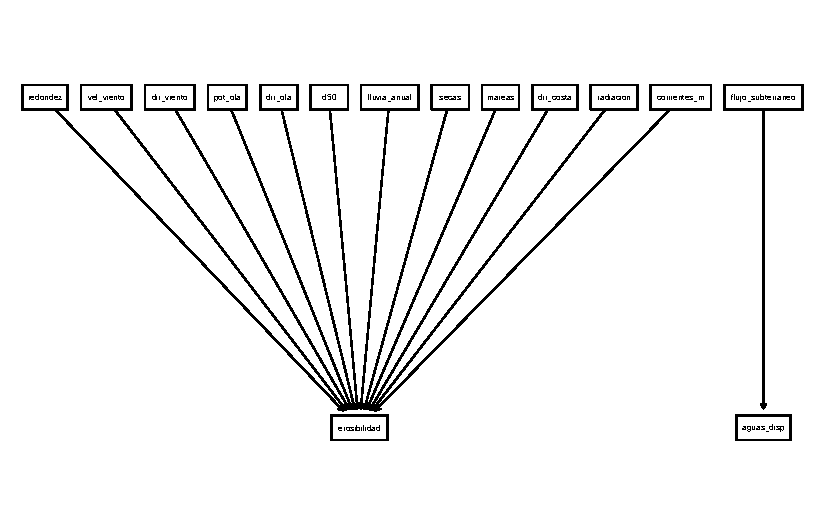
\includegraphics{capitulos/miro-costas_files/figure-pdf/unnamed-chunk-4-1.pdf}

}

\end{figure}

La lista de variables identificadas es:

\global\setlength{\Oldarrayrulewidth}{\arrayrulewidth}

\global\setlength{\Oldtabcolsep}{\tabcolsep}

\setlength{\tabcolsep}{2pt}

\renewcommand*{\arraystretch}{1.5}



\providecommand{\ascline}[3]{\noalign{\global\arrayrulewidth #1}\arrayrulecolor[HTML]{#2}\cline{#3}}

\begin{longtable*}[c]{|p{0.75in}|p{0.75in}|p{0.75in}}



\ascline{1.5pt}{666666}{1-3}

\multicolumn{1}{>{\raggedright}m{\dimexpr 0.75in+0\tabcolsep}}{\textcolor[HTML]{000000}{\fontsize{8}{8}\selectfont{\global\setmainfont{Arial}{text}}}} & \multicolumn{1}{>{\raggedright}m{\dimexpr 0.75in+0\tabcolsep}}{\textcolor[HTML]{000000}{\fontsize{8}{8}\selectfont{\global\setmainfont{Arial}{var}}}} & \multicolumn{1}{>{\raggedright}m{\dimexpr 0.75in+0\tabcolsep}}{\textcolor[HTML]{000000}{\fontsize{8}{8}\selectfont{\global\setmainfont{Arial}{color}}}} \\

\ascline{1.5pt}{666666}{1-3}\endfirsthead 

\ascline{1.5pt}{666666}{1-3}

\multicolumn{1}{>{\raggedright}m{\dimexpr 0.75in+0\tabcolsep}}{\textcolor[HTML]{000000}{\fontsize{8}{8}\selectfont{\global\setmainfont{Arial}{text}}}} & \multicolumn{1}{>{\raggedright}m{\dimexpr 0.75in+0\tabcolsep}}{\textcolor[HTML]{000000}{\fontsize{8}{8}\selectfont{\global\setmainfont{Arial}{var}}}} & \multicolumn{1}{>{\raggedright}m{\dimexpr 0.75in+0\tabcolsep}}{\textcolor[HTML]{000000}{\fontsize{8}{8}\selectfont{\global\setmainfont{Arial}{color}}}} \\

\ascline{1.5pt}{666666}{1-3}\endhead



\multicolumn{1}{>{\raggedright}m{\dimexpr 0.75in+0\tabcolsep}}{\textcolor[HTML]{000000}{\fontsize{8}{8}\selectfont{\global\setmainfont{Arial}{potencia\ de\ la\ ola\ (datos\ horarios\ 1940-2022)https://confluence.ecmwf.int/display/CKB/ERA5\%3A\&\#43;data\&\#43;documentation}}}} & \multicolumn{1}{>{\raggedright}m{\dimexpr 0.75in+0\tabcolsep}}{\textcolor[HTML]{000000}{\fontsize{8}{8}\selectfont{\global\setmainfont{Arial}{pot\_ola}}}} & \multicolumn{1}{>{\raggedright}m{\dimexpr 0.75in+0\tabcolsep}}{\textcolor[HTML]{000000}{\fontsize{8}{8}\selectfont{\global\setmainfont{Arial}{blue}}}} \\





\multicolumn{1}{>{\raggedright}m{\dimexpr 0.75in+0\tabcolsep}}{\textcolor[HTML]{000000}{\fontsize{8}{8}\selectfont{\global\setmainfont{Arial}{mareasMareografos\ de\ Pafícico\ y\ Atlántico\ (SEMAR)\ RODOLFO}}}} & \multicolumn{1}{>{\raggedright}m{\dimexpr 0.75in+0\tabcolsep}}{\textcolor[HTML]{000000}{\fontsize{8}{8}\selectfont{\global\setmainfont{Arial}{mareas}}}} & \multicolumn{1}{>{\raggedright}m{\dimexpr 0.75in+0\tabcolsep}}{\textcolor[HTML]{000000}{\fontsize{8}{8}\selectfont{\global\setmainfont{Arial}{blue}}}} \\





\multicolumn{1}{>{\raggedright}m{\dimexpr 0.75in+0\tabcolsep}}{\textcolor[HTML]{000000}{\fontsize{8}{8}\selectfont{\global\setmainfont{Arial}{forma\ de\ crecimiento\ de\ vegetación\ de\ dunas:Tomar\ de\ base\ de\ datos\ de\ Ileana/conabio.\ Zonas\ con\ arbustivas\ tienden\ mayor\ erosión.\ en\ zonas\ como\ dice\ marisa\ eso\ no\ pasa}}}} & \multicolumn{1}{>{\raggedright}m{\dimexpr 0.75in+0\tabcolsep}}{\textcolor[HTML]{000000}{\fontsize{8}{8}\selectfont{\global\setmainfont{Arial}{habito}}}} & \multicolumn{1}{>{\raggedright}m{\dimexpr 0.75in+0\tabcolsep}}{\textcolor[HTML]{000000}{\fontsize{8}{8}\selectfont{\global\setmainfont{Arial}{dark\_green}}}} \\





\multicolumn{1}{>{\raggedright}m{\dimexpr 0.75in+0\tabcolsep}}{\textcolor[HTML]{000000}{\fontsize{8}{8}\selectfont{\global\setmainfont{Arial}{disponinibilidad\ de\ arena\ -ancho\ playa}}}} & \multicolumn{1}{>{\raggedright}m{\dimexpr 0.75in+0\tabcolsep}}{\textcolor[HTML]{000000}{\fontsize{8}{8}\selectfont{\global\setmainfont{Arial}{ancho\_playa}}}} & \multicolumn{1}{>{\raggedright}m{\dimexpr 0.75in+0\tabcolsep}}{\textcolor[HTML]{000000}{\fontsize{8}{8}\selectfont{\global\setmainfont{Arial}{dark\_green}}}} \\





\multicolumn{1}{>{\raggedright}m{\dimexpr 0.75in+0\tabcolsep}}{\textcolor[HTML]{000000}{\fontsize{8}{8}\selectfont{\global\setmainfont{Arial}{geología(geomorfología,tipo\ de\ roca)Pedir\ carta\ geológica\ minera\ servicio\ geologico\ mexicano.\ Octavio\ \ y\ Karla\ en\ formato\ shape\ \&\#34;Geológica\ minera\&\#34;https://www.sgm.gob.mx/CartasDisponibles/\ (en\ pdf\ hasta\ 1:50000)https://www.sgm.gob.mx/GeoInfoMexGobMx/\#(shape)}}}} & \multicolumn{1}{>{\raggedright}m{\dimexpr 0.75in+0\tabcolsep}}{\textcolor[HTML]{000000}{\fontsize{8}{8}\selectfont{\global\setmainfont{Arial}{geologia}}}} & \multicolumn{1}{>{\raggedright}m{\dimexpr 0.75in+0\tabcolsep}}{\textcolor[HTML]{000000}{\fontsize{8}{8}\selectfont{\global\setmainfont{Arial}{blue}}}} \\





\multicolumn{1}{>{\raggedright}m{\dimexpr 0.75in+0\tabcolsep}}{\textcolor[HTML]{000000}{\fontsize{8}{8}\selectfont{\global\setmainfont{Arial}{Arrecifes\ de\ coral-Buscar\ la\ mejor\ capa:\ blaqueamiento,\ Copernicus\ o\ Conabiohttps://simar.conabio.gob.mx/explorer/?undefined}}}} & \multicolumn{1}{>{\raggedright}m{\dimexpr 0.75in+0\tabcolsep}}{\textcolor[HTML]{000000}{\fontsize{8}{8}\selectfont{\global\setmainfont{Arial}{coral}}}} & \multicolumn{1}{>{\raggedright}m{\dimexpr 0.75in+0\tabcolsep}}{\textcolor[HTML]{000000}{\fontsize{8}{8}\selectfont{\global\setmainfont{Arial}{dark\_green}}}} \\





\multicolumn{1}{>{\raggedright}m{\dimexpr 0.75in+0\tabcolsep}}{\textcolor[HTML]{000000}{\fontsize{8}{8}\selectfont{\global\setmainfont{Arial}{pastos\ marinoshttps://simar.conabio.gob.mx/explorer/?undefined}}}} & \multicolumn{1}{>{\raggedright}m{\dimexpr 0.75in+0\tabcolsep}}{\textcolor[HTML]{000000}{\fontsize{8}{8}\selectfont{\global\setmainfont{Arial}{pastos}}}} & \multicolumn{1}{>{\raggedright}m{\dimexpr 0.75in+0\tabcolsep}}{\textcolor[HTML]{000000}{\fontsize{8}{8}\selectfont{\global\setmainfont{Arial}{dark\_green}}}} \\





\multicolumn{1}{>{\raggedright}m{\dimexpr 0.75in+0\tabcolsep}}{\textcolor[HTML]{000000}{\fontsize{8}{8}\selectfont{\global\setmainfont{Arial}{Disponibilidad\ de\ agua\ salobre\ o\ dulce}}}} & \multicolumn{1}{>{\raggedright}m{\dimexpr 0.75in+0\tabcolsep}}{\textcolor[HTML]{000000}{\fontsize{8}{8}\selectfont{\global\setmainfont{Arial}{aguas\_disp}}}} & \multicolumn{1}{>{\raggedright}m{\dimexpr 0.75in+0\tabcolsep}}{\textcolor[HTML]{000000}{\fontsize{8}{8}\selectfont{\global\setmainfont{Arial}{blue}}}} \\





\multicolumn{1}{>{\raggedright}m{\dimexpr 0.75in+0\tabcolsep}}{\textcolor[HTML]{000000}{\fontsize{8}{8}\selectfont{\global\setmainfont{Arial}{Flujo\ subterráneo.\ Información\ disponible\ en\ SHP\ (polígonos).\ Solicitar\ a Rodolfo\ / Valeria.\ Tiene\ una\ clasificación.\ Nivel\ nacional.\ Artículo:\ https://www.mdpi.com/2073-4441/12/9/2459}}}} & \multicolumn{1}{>{\raggedright}m{\dimexpr 0.75in+0\tabcolsep}}{\textcolor[HTML]{000000}{\fontsize{8}{8}\selectfont{\global\setmainfont{Arial}{flujo\_subterraneo}}}} & \multicolumn{1}{>{\raggedright}m{\dimexpr 0.75in+0\tabcolsep}}{\textcolor[HTML]{000000}{\fontsize{8}{8}\selectfont{\global\setmainfont{Arial}{blue}}}} \\





\multicolumn{1}{>{\raggedright}m{\dimexpr 0.75in+0\tabcolsep}}{\textcolor[HTML]{000000}{\fontsize{8}{8}\selectfont{\global\setmainfont{Arial}{Sol.\ WB\_Global\ solar\ atlas.\ https://globalsolaratlas.info/map?c\&\#61;19.248922,-97.171326,9\&amp;s\&\#61;19.519781,-96.911168\&amp;m\&\#61;site\ }}}} & \multicolumn{1}{>{\raggedright}m{\dimexpr 0.75in+0\tabcolsep}}{\textcolor[HTML]{000000}{\fontsize{8}{8}\selectfont{\global\setmainfont{Arial}{radiacion}}}} & \multicolumn{1}{>{\raggedright}m{\dimexpr 0.75in+0\tabcolsep}}{\textcolor[HTML]{000000}{\fontsize{8}{8}\selectfont{\global\setmainfont{Arial}{blue}}}} \\





\multicolumn{1}{>{\raggedright}m{\dimexpr 0.75in+0\tabcolsep}}{\textcolor[HTML]{000000}{\fontsize{8}{8}\selectfont{\global\setmainfont{Arial}{EvapotraspiraciónEn\ terminos\ de\ germinación\ y\ cobertura}}}} & \multicolumn{1}{>{\raggedright}m{\dimexpr 0.75in+0\tabcolsep}}{\textcolor[HTML]{000000}{\fontsize{8}{8}\selectfont{\global\setmainfont{Arial}{evapotranspiracion}}}} & \multicolumn{1}{>{\raggedright}m{\dimexpr 0.75in+0\tabcolsep}}{\textcolor[HTML]{000000}{\fontsize{8}{8}\selectfont{\global\setmainfont{Arial}{dark\_green}}}} \\





\multicolumn{1}{>{\raggedright}m{\dimexpr 0.75in+0\tabcolsep}}{\textcolor[HTML]{000000}{\fontsize{8}{8}\selectfont{\global\setmainfont{Arial}{NOTAS\ GENERALESJuntaremos\ playa\ y\ duna\ como\ un\ solo\ ecosistema.\ Sugerencia\ de\ Rodolfo}}}} & \multicolumn{1}{>{\raggedright}m{\dimexpr 0.75in+0\tabcolsep}}{\textcolor[HTML]{000000}{\fontsize{8}{8}\selectfont{\global\setmainfont{Arial}{notas\_1}}}} & \multicolumn{1}{>{\raggedright}m{\dimexpr 0.75in+0\tabcolsep}}{\textcolor[HTML]{000000}{\fontsize{8}{8}\selectfont{\global\setmainfont{Arial}{gray}}}} \\





\multicolumn{1}{>{\raggedright}m{\dimexpr 0.75in+0\tabcolsep}}{\textcolor[HTML]{000000}{\fontsize{8}{8}\selectfont{\global\setmainfont{Arial}{Plataforma\ continental.\ GEBCO.\ Gridded\ Bathymetry\ data\ download.https://download.gebco.net}}}} & \multicolumn{1}{>{\raggedright}m{\dimexpr 0.75in+0\tabcolsep}}{\textcolor[HTML]{000000}{\fontsize{8}{8}\selectfont{\global\setmainfont{Arial}{plataforma\_cont}}}} & \multicolumn{1}{>{\raggedright}m{\dimexpr 0.75in+0\tabcolsep}}{\textcolor[HTML]{000000}{\fontsize{8}{8}\selectfont{\global\setmainfont{Arial}{blue}}}} \\





\multicolumn{1}{>{\raggedright}m{\dimexpr 0.75in+0\tabcolsep}}{\textcolor[HTML]{000000}{\fontsize{8}{8}\selectfont{\global\setmainfont{Arial}{Infraestructura}}}} & \multicolumn{1}{>{\raggedright}m{\dimexpr 0.75in+0\tabcolsep}}{\textcolor[HTML]{000000}{\fontsize{8}{8}\selectfont{\global\setmainfont{Arial}{infraestruct}}}} & \multicolumn{1}{>{\raggedright}m{\dimexpr 0.75in+0\tabcolsep}}{\textcolor[HTML]{000000}{\fontsize{8}{8}\selectfont{\global\setmainfont{Arial}{orange}}}} \\





\multicolumn{1}{>{\raggedright}m{\dimexpr 0.75in+0\tabcolsep}}{\textcolor[HTML]{000000}{\fontsize{8}{8}\selectfont{\global\setmainfont{Arial}{ManglaresSIMARPaty\ Moreno}}}} & \multicolumn{1}{>{\raggedright}m{\dimexpr 0.75in+0\tabcolsep}}{\textcolor[HTML]{000000}{\fontsize{8}{8}\selectfont{\global\setmainfont{Arial}{mangle}}}} & \multicolumn{1}{>{\raggedright}m{\dimexpr 0.75in+0\tabcolsep}}{\textcolor[HTML]{000000}{\fontsize{8}{8}\selectfont{\global\setmainfont{Arial}{dark\_green}}}} \\





\multicolumn{1}{>{\raggedright}m{\dimexpr 0.75in+0\tabcolsep}}{\textcolor[HTML]{000000}{\fontsize{8}{8}\selectfont{\global\setmainfont{Arial}{Estructuras\ marinas}}}} & \multicolumn{1}{>{\raggedright}m{\dimexpr 0.75in+0\tabcolsep}}{\textcolor[HTML]{000000}{\fontsize{8}{8}\selectfont{\global\setmainfont{Arial}{estruct\_marina}}}} & \multicolumn{1}{>{\raggedright}m{\dimexpr 0.75in+0\tabcolsep}}{\textcolor[HTML]{000000}{\fontsize{8}{8}\selectfont{\global\setmainfont{Arial}{orange}}}} \\





\multicolumn{1}{>{\raggedright}m{\dimexpr 0.75in+0\tabcolsep}}{\textcolor[HTML]{000000}{\fontsize{8}{8}\selectfont{\global\setmainfont{Arial}{Influencia\ antrópica}}}} & \multicolumn{1}{>{\raggedright}m{\dimexpr 0.75in+0\tabcolsep}}{\textcolor[HTML]{000000}{\fontsize{8}{8}\selectfont{\global\setmainfont{Arial}{influ\_antro}}}} & \multicolumn{1}{>{\raggedright}m{\dimexpr 0.75in+0\tabcolsep}}{\textcolor[HTML]{000000}{\fontsize{8}{8}\selectfont{\global\setmainfont{Arial}{orange}}}} \\





\multicolumn{1}{>{\raggedright}m{\dimexpr 0.75in+0\tabcolsep}}{\textcolor[HTML]{000000}{\fontsize{8}{8}\selectfont{\global\setmainfont{Arial}{ALTERACIONES\ ANTROPICAS\ DE\ LA\ Calidad\ del\ agua}}}} & \multicolumn{1}{>{\raggedright}m{\dimexpr 0.75in+0\tabcolsep}}{\textcolor[HTML]{000000}{\fontsize{8}{8}\selectfont{\global\setmainfont{Arial}{alt\_antro}}}} & \multicolumn{1}{>{\raggedright}m{\dimexpr 0.75in+0\tabcolsep}}{\textcolor[HTML]{000000}{\fontsize{8}{8}\selectfont{\global\setmainfont{Arial}{orange}}}} \\





\multicolumn{1}{>{\raggedright}m{\dimexpr 0.75in+0\tabcolsep}}{\textcolor[HTML]{000000}{\fontsize{8}{8}\selectfont{\global\setmainfont{Arial}{Pendiente\ de\ la\ playaInformación\ puntualMónica\ y\ otros}}}} & \multicolumn{1}{>{\raggedright}m{\dimexpr 0.75in+0\tabcolsep}}{\textcolor[HTML]{000000}{\fontsize{8}{8}\selectfont{\global\setmainfont{Arial}{pendiente}}}} & \multicolumn{1}{>{\raggedright}m{\dimexpr 0.75in+0\tabcolsep}}{\textcolor[HTML]{000000}{\fontsize{8}{8}\selectfont{\global\setmainfont{Arial}{dark\_green}}}} \\





\multicolumn{1}{>{\raggedright}m{\dimexpr 0.75in+0\tabcolsep}}{\textcolor[HTML]{000000}{\fontsize{8}{8}\selectfont{\global\setmainfont{Arial}{Diámetro\ mediano\ D50(base\ de\ datos\ GICP-IIUNAM)}}}} & \multicolumn{1}{>{\raggedright}m{\dimexpr 0.75in+0\tabcolsep}}{\textcolor[HTML]{000000}{\fontsize{8}{8}\selectfont{\global\setmainfont{Arial}{d50}}}} & \multicolumn{1}{>{\raggedright}m{\dimexpr 0.75in+0\tabcolsep}}{\textcolor[HTML]{000000}{\fontsize{8}{8}\selectfont{\global\setmainfont{Arial}{blue}}}} \\





\multicolumn{1}{>{\raggedright}m{\dimexpr 0.75in+0\tabcolsep}}{\textcolor[HTML]{000000}{\fontsize{8}{8}\selectfont{\global\setmainfont{Arial}{Redondez\ sedimento.\ (base\ de\ datos\ GICP-IIUNAM)}}}} & \multicolumn{1}{>{\raggedright}m{\dimexpr 0.75in+0\tabcolsep}}{\textcolor[HTML]{000000}{\fontsize{8}{8}\selectfont{\global\setmainfont{Arial}{redondez}}}} & \multicolumn{1}{>{\raggedright}m{\dimexpr 0.75in+0\tabcolsep}}{\textcolor[HTML]{000000}{\fontsize{8}{8}\selectfont{\global\setmainfont{Arial}{blue}}}} \\





\multicolumn{1}{>{\raggedright}m{\dimexpr 0.75in+0\tabcolsep}}{\textcolor[HTML]{000000}{\fontsize{8}{8}\selectfont{\global\setmainfont{Arial}{Dirección\ de\ la\ línea\ de\ costa\ con\ relación\ al\ oleaje\ y\ al\ vientoUsar\ línea\ de\ costa\ propuesta\ por\ \ Rodolfo}}}} & \multicolumn{1}{>{\raggedright}m{\dimexpr 0.75in+0\tabcolsep}}{\textcolor[HTML]{000000}{\fontsize{8}{8}\selectfont{\global\setmainfont{Arial}{dir\_costa}}}} & \multicolumn{1}{>{\raggedright}m{\dimexpr 0.75in+0\tabcolsep}}{\textcolor[HTML]{000000}{\fontsize{8}{8}\selectfont{\global\setmainfont{Arial}{blue}}}} \\





\multicolumn{1}{>{\raggedright}m{\dimexpr 0.75in+0\tabcolsep}}{\textcolor[HTML]{000000}{\fontsize{8}{8}\selectfont{\global\setmainfont{Arial}{Efecto\ del\ sargazo}}}} & \multicolumn{1}{>{\raggedright}m{\dimexpr 0.75in+0\tabcolsep}}{\textcolor[HTML]{000000}{\fontsize{8}{8}\selectfont{\global\setmainfont{Arial}{EfectoDelSargaso}}}} & \multicolumn{1}{>{\raggedright}m{\dimexpr 0.75in+0\tabcolsep}}{\textcolor[HTML]{000000}{\fontsize{8}{8}\selectfont{\global\setmainfont{Arial}{violet}}}} \\





\multicolumn{1}{>{\raggedright}m{\dimexpr 0.75in+0\tabcolsep}}{\textcolor[HTML]{000000}{\fontsize{8}{8}\selectfont{\global\setmainfont{Arial}{Corrientes\ MarinasAtlas\ de\ corrientes\ IMTA\ de\ Efraín\ Mateos\ (Base\ de\ datos\ del\ CEMIE)VALERIA}}}} & \multicolumn{1}{>{\raggedright}m{\dimexpr 0.75in+0\tabcolsep}}{\textcolor[HTML]{000000}{\fontsize{8}{8}\selectfont{\global\setmainfont{Arial}{corrientes\_m}}}} & \multicolumn{1}{>{\raggedright}m{\dimexpr 0.75in+0\tabcolsep}}{\textcolor[HTML]{000000}{\fontsize{8}{8}\selectfont{\global\setmainfont{Arial}{blue}}}} \\





\multicolumn{1}{>{\raggedright}m{\dimexpr 0.75in+0\tabcolsep}}{\textcolor[HTML]{000000}{\fontsize{8}{8}\selectfont{\global\setmainfont{Arial}{Especies\ invasorasUsar\ datos\ procesados\ por\ Julián}}}} & \multicolumn{1}{>{\raggedright}m{\dimexpr 0.75in+0\tabcolsep}}{\textcolor[HTML]{000000}{\fontsize{8}{8}\selectfont{\global\setmainfont{Arial}{invasoras}}}} & \multicolumn{1}{>{\raggedright}m{\dimexpr 0.75in+0\tabcolsep}}{\textcolor[HTML]{000000}{\fontsize{8}{8}\selectfont{\global\setmainfont{Arial}{dark\_green}}}} \\





\multicolumn{1}{>{\raggedright}m{\dimexpr 0.75in+0\tabcolsep}}{\textcolor[HTML]{000000}{\fontsize{8}{8}\selectfont{\global\setmainfont{Arial}{Perfil\ de\ sueloPerfiles\ edafológicos\ se\ pueden\ encontrar\ en:https://www.inegi.org.mx/app/biblioteca/ficha.html?upc\&\#61;702825266707Suelos\ sueltos\ y\ poco\ compactados\ son\ más\ susceptibles\ a\ la\ erosión\ eólica,\ lo\ que\ facilita\ la\ formación\ de\ dunas.\ Por\ otro\ lado,\ suelos\ más\ compactos\ pueden\ resistir\ mejor\ la\ acción\ del\ viento.\ La\ presencia\ de\ diferentes\ horizontes\ en\ el\ perfil\ edafológico\ puede\ afectar\ la\ disponibilidad\ de\ sedimentos\ para\ la\ formación\ de\ dunas.\ Un\ horizonte\ superficial\ arenoso\ es\ ideal\ para\ la\ movilización\ de\ partículas.}}}} & \multicolumn{1}{>{\raggedright}m{\dimexpr 0.75in+0\tabcolsep}}{\textcolor[HTML]{000000}{\fontsize{8}{8}\selectfont{\global\setmainfont{Arial}{perfilsuelo}}}} & \multicolumn{1}{>{\raggedright}m{\dimexpr 0.75in+0\tabcolsep}}{\textcolor[HTML]{000000}{\fontsize{8}{8}\selectfont{\global\setmainfont{Arial}{dark\_green}}}} \\





\multicolumn{1}{>{\raggedright}m{\dimexpr 0.75in+0\tabcolsep}}{\textcolor[HTML]{000000}{\fontsize{8}{8}\selectfont{\global\setmainfont{Arial}{Macroalgashttps://fjps.springeropen.com/articles/10.1186/s43094-020-00147-6}}}} & \multicolumn{1}{>{\raggedright}m{\dimexpr 0.75in+0\tabcolsep}}{\textcolor[HTML]{000000}{\fontsize{8}{8}\selectfont{\global\setmainfont{Arial}{macroalgas}}}} & \multicolumn{1}{>{\raggedright}m{\dimexpr 0.75in+0\tabcolsep}}{\textcolor[HTML]{000000}{\fontsize{8}{8}\selectfont{\global\setmainfont{Arial}{dark\_green}}}} \\





\multicolumn{1}{>{\raggedright}m{\dimexpr 0.75in+0\tabcolsep}}{\textcolor[HTML]{000000}{\fontsize{8}{8}\selectfont{\global\setmainfont{Arial}{Estacionalidad\ fuente:\ copernicus.\ posprocesar\ para\ ver\ también\ temporada\ de\ secas\ VALERIA\ -\ Marisa\ proporciona\ el\ criterio}}}} & \multicolumn{1}{>{\raggedright}m{\dimexpr 0.75in+0\tabcolsep}}{\textcolor[HTML]{000000}{\fontsize{8}{8}\selectfont{\global\setmainfont{Arial}{secas}}}} & \multicolumn{1}{>{\raggedright}m{\dimexpr 0.75in+0\tabcolsep}}{\textcolor[HTML]{000000}{\fontsize{8}{8}\selectfont{\global\setmainfont{Arial}{blue}}}} \\





\multicolumn{1}{>{\raggedright}m{\dimexpr 0.75in+0\tabcolsep}}{\textcolor[HTML]{000000}{\fontsize{8}{8}\selectfont{\global\setmainfont{Arial}{Condición}}}} & \multicolumn{1}{>{\raggedright}m{\dimexpr 0.75in+0\tabcolsep}}{\textcolor[HTML]{000000}{\fontsize{8}{8}\selectfont{\global\setmainfont{Arial}{condicion}}}} & \multicolumn{1}{>{\raggedright}m{\dimexpr 0.75in+0\tabcolsep}}{\textcolor[HTML]{000000}{\fontsize{8}{8}\selectfont{\global\setmainfont{Arial}{green}}}} \\





\multicolumn{1}{>{\raggedright}m{\dimexpr 0.75in+0\tabcolsep}}{\textcolor[HTML]{000000}{\fontsize{8}{8}\selectfont{\global\setmainfont{Arial}{Precipitación-\ fuente:\ copernicus.\ posprocesar\ para\ ver\ también\ temporada\ de\ secas\ VALERIA}}}} & \multicolumn{1}{>{\raggedright}m{\dimexpr 0.75in+0\tabcolsep}}{\textcolor[HTML]{000000}{\fontsize{8}{8}\selectfont{\global\setmainfont{Arial}{lluvia\_anual}}}} & \multicolumn{1}{>{\raggedright}m{\dimexpr 0.75in+0\tabcolsep}}{\textcolor[HTML]{000000}{\fontsize{8}{8}\selectfont{\global\setmainfont{Arial}{blue}}}} \\





\multicolumn{1}{>{\raggedright}m{\dimexpr 0.75in+0\tabcolsep}}{\textcolor[HTML]{000000}{\fontsize{8}{8}\selectfont{\global\setmainfont{Arial}{GastoEscurrimiento\ en\ cuencaAporte\ de\ sedimento\ terrígeno}}}} & \multicolumn{1}{>{\raggedright}m{\dimexpr 0.75in+0\tabcolsep}}{\textcolor[HTML]{000000}{\fontsize{8}{8}\selectfont{\global\setmainfont{Arial}{gasto}}}} & \multicolumn{1}{>{\raggedright}m{\dimexpr 0.75in+0\tabcolsep}}{\textcolor[HTML]{000000}{\fontsize{8}{8}\selectfont{\global\setmainfont{Arial}{blue}}}} \\





\multicolumn{1}{>{\raggedright}m{\dimexpr 0.75in+0\tabcolsep}}{\textcolor[HTML]{000000}{\fontsize{8}{8}\selectfont{\global\setmainfont{Arial}{dirección\ de\ la\ ola\ (datos\ horarios\ 1940-2022)https://confluence.ecmwf.int/display/CKB/ERA5\%3A\&\#43;data\&\#43;documentation}}}} & \multicolumn{1}{>{\raggedright}m{\dimexpr 0.75in+0\tabcolsep}}{\textcolor[HTML]{000000}{\fontsize{8}{8}\selectfont{\global\setmainfont{Arial}{dir\_ola}}}} & \multicolumn{1}{>{\raggedright}m{\dimexpr 0.75in+0\tabcolsep}}{\textcolor[HTML]{000000}{\fontsize{8}{8}\selectfont{\global\setmainfont{Arial}{blue}}}} \\





\multicolumn{1}{>{\raggedright}m{\dimexpr 0.75in+0\tabcolsep}}{\textcolor[HTML]{000000}{\fontsize{8}{8}\selectfont{\global\setmainfont{Arial}{velocidad\ del\ viento (datos\ horarios\ 1940-2022)https://confluence.ecmwf.int/display/CKB/ERA5\%3A\&\#43;data\&\#43;documentationEventos\ de\ vientos\ extremos.\ Encontrar\ umbrales\ de\ viento\ y\ ver\ si\ favorecen\ la\ construcción\ o\ la\ destrucción\ de\ duna.\ ¿Velocidad\ de\ inicio\ de\ arrastre?WB\_Atlas\ eólico\ mundial:\ https://globalwindatlas.info/es/PENDIENTE\ DEFINIR\ UMBRALES}}}} & \multicolumn{1}{>{\raggedright}m{\dimexpr 0.75in+0\tabcolsep}}{\textcolor[HTML]{000000}{\fontsize{8}{8}\selectfont{\global\setmainfont{Arial}{vel\_viento}}}} & \multicolumn{1}{>{\raggedright}m{\dimexpr 0.75in+0\tabcolsep}}{\textcolor[HTML]{000000}{\fontsize{8}{8}\selectfont{\global\setmainfont{Arial}{blue}}}} \\





\multicolumn{1}{>{\raggedright}m{\dimexpr 0.75in+0\tabcolsep}}{\textcolor[HTML]{000000}{\fontsize{8}{8}\selectfont{\global\setmainfont{Arial}{dirección\ del\ viento (datos\ horarios\ 1940-2022)https://confluence.ecmwf.int/display/CKB/ERA5\%3A\&\#43;data\&\#43;documentation}}}} & \multicolumn{1}{>{\raggedright}m{\dimexpr 0.75in+0\tabcolsep}}{\textcolor[HTML]{000000}{\fontsize{8}{8}\selectfont{\global\setmainfont{Arial}{dir\_viento}}}} & \multicolumn{1}{>{\raggedright}m{\dimexpr 0.75in+0\tabcolsep}}{\textcolor[HTML]{000000}{\fontsize{8}{8}\selectfont{\global\setmainfont{Arial}{blue}}}} \\





\multicolumn{1}{>{\raggedright}m{\dimexpr 0.75in+0\tabcolsep}}{\textcolor[HTML]{000000}{\fontsize{8}{8}\selectfont{\global\setmainfont{Arial}{Detección}}}} & \multicolumn{1}{>{\raggedright}m{\dimexpr 0.75in+0\tabcolsep}}{\textcolor[HTML]{000000}{\fontsize{8}{8}\selectfont{\global\setmainfont{Arial}{inf\_2}}}} & \multicolumn{1}{>{\raggedright}m{\dimexpr 0.75in+0\tabcolsep}}{\textcolor[HTML]{000000}{\fontsize{8}{8}\selectfont{\global\setmainfont{Arial}{dark\_green}}}} \\





\multicolumn{1}{>{\raggedright}m{\dimexpr 0.75in+0\tabcolsep}}{\textcolor[HTML]{000000}{\fontsize{8}{8}\selectfont{\global\setmainfont{Arial}{Contexto}}}} & \multicolumn{1}{>{\raggedright}m{\dimexpr 0.75in+0\tabcolsep}}{\textcolor[HTML]{000000}{\fontsize{8}{8}\selectfont{\global\setmainfont{Arial}{inf\_1}}}} & \multicolumn{1}{>{\raggedright}m{\dimexpr 0.75in+0\tabcolsep}}{\textcolor[HTML]{000000}{\fontsize{8}{8}\selectfont{\global\setmainfont{Arial}{blue}}}} \\





\multicolumn{1}{>{\raggedright}m{\dimexpr 0.75in+0\tabcolsep}}{\textcolor[HTML]{000000}{\fontsize{8}{8}\selectfont{\global\setmainfont{Arial}{Otro}}}} & \multicolumn{1}{>{\raggedright}m{\dimexpr 0.75in+0\tabcolsep}}{\textcolor[HTML]{000000}{\fontsize{8}{8}\selectfont{\global\setmainfont{Arial}{inf\_4}}}} & \multicolumn{1}{>{\raggedright}m{\dimexpr 0.75in+0\tabcolsep}}{\textcolor[HTML]{000000}{\fontsize{8}{8}\selectfont{\global\setmainfont{Arial}{violet}}}} \\





\multicolumn{1}{>{\raggedright}m{\dimexpr 0.75in+0\tabcolsep}}{\textcolor[HTML]{000000}{\fontsize{8}{8}\selectfont{\global\setmainfont{Arial}{Intervención\ hunama}}}} & \multicolumn{1}{>{\raggedright}m{\dimexpr 0.75in+0\tabcolsep}}{\textcolor[HTML]{000000}{\fontsize{8}{8}\selectfont{\global\setmainfont{Arial}{inf\_3}}}} & \multicolumn{1}{>{\raggedright}m{\dimexpr 0.75in+0\tabcolsep}}{\textcolor[HTML]{000000}{\fontsize{8}{8}\selectfont{\global\setmainfont{Arial}{orange}}}} \\





\multicolumn{1}{>{\raggedright}m{\dimexpr 0.75in+0\tabcolsep}}{\textcolor[HTML]{000000}{\fontsize{8}{8}\selectfont{\global\setmainfont{Arial}{HumedadEn\ terminos\ de\ germinación\ y\ cobertura}}}} & \multicolumn{1}{>{\raggedright}m{\dimexpr 0.75in+0\tabcolsep}}{\textcolor[HTML]{000000}{\fontsize{8}{8}\selectfont{\global\setmainfont{Arial}{humedad}}}} & \multicolumn{1}{>{\raggedright}m{\dimexpr 0.75in+0\tabcolsep}}{\textcolor[HTML]{000000}{\fontsize{8}{8}\selectfont{\global\setmainfont{Arial}{dark\_green}}}} \\





\multicolumn{1}{>{\raggedright}m{\dimexpr 0.75in+0\tabcolsep}}{\textcolor[HTML]{000000}{\fontsize{8}{8}\selectfont{\global\setmainfont{Arial}{Checar\ pagina\ de\ idea\ del\ instituto\ de\ geografíahttps://www.gits.igg.unam.mx/idea/descargaGaby\ Gómez}}}} & \multicolumn{1}{>{\raggedright}m{\dimexpr 0.75in+0\tabcolsep}}{\textcolor[HTML]{000000}{\fontsize{8}{8}\selectfont{\global\setmainfont{Arial}{notas\_2}}}} & \multicolumn{1}{>{\raggedright}m{\dimexpr 0.75in+0\tabcolsep}}{\textcolor[HTML]{000000}{\fontsize{8}{8}\selectfont{\global\setmainfont{Arial}{gray}}}} \\





\multicolumn{1}{>{\raggedright}m{\dimexpr 0.75in+0\tabcolsep}}{\textcolor[HTML]{000000}{\fontsize{8}{8}\selectfont{\global\setmainfont{Arial}{Tasa\ de\ desplazamiento(Erosión-\ /\ acresión\ \&\#43;)}}}} & \multicolumn{1}{>{\raggedright}m{\dimexpr 0.75in+0\tabcolsep}}{\textcolor[HTML]{000000}{\fontsize{8}{8}\selectfont{\global\setmainfont{Arial}{-}}}} & \multicolumn{1}{>{\raggedright}m{\dimexpr 0.75in+0\tabcolsep}}{\textcolor[HTML]{000000}{\fontsize{8}{8}\selectfont{\global\setmainfont{Arial}{dark\_green}}}} \\





\multicolumn{1}{>{\raggedright}m{\dimexpr 0.75in+0\tabcolsep}}{\textcolor[HTML]{000000}{\fontsize{8}{8}\selectfont{\global\setmainfont{Arial}{erosibilidad}}}} & \multicolumn{1}{>{\raggedright}m{\dimexpr 0.75in+0\tabcolsep}}{\textcolor[HTML]{000000}{\fontsize{8}{8}\selectfont{\global\setmainfont{Arial}{erosibilidad}}}} & \multicolumn{1}{>{\raggedright}m{\dimexpr 0.75in+0\tabcolsep}}{\textcolor[HTML]{000000}{\fontsize{8}{8}\selectfont{\global\setmainfont{Arial}{green}}}} \\





\multicolumn{1}{>{\raggedright}m{\dimexpr 0.75in+0\tabcolsep}}{\textcolor[HTML]{000000}{\fontsize{8}{8}\selectfont{\global\setmainfont{Arial}{Resolución\ raster100\ m\ por\ lado\ (equivalete\ a\ 3\ segundos)En\ versión\ \&\#34;caso\ de\ estudio\&\#34;\ serán\ pixeles\ de\ 10m\ por\ lado\ (equivale\ a\ 0.3\ segundos).}}}} & \multicolumn{1}{>{\raggedright}m{\dimexpr 0.75in+0\tabcolsep}}{\textcolor[HTML]{000000}{\fontsize{8}{8}\selectfont{\global\setmainfont{Arial}{resolucion}}}} & \multicolumn{1}{>{\raggedright}m{\dimexpr 0.75in+0\tabcolsep}}{\textcolor[HTML]{000000}{\fontsize{8}{8}\selectfont{\global\setmainfont{Arial}{cyan}}}} \\





\multicolumn{1}{>{\raggedright}m{\dimexpr 0.75in+0\tabcolsep}}{\textcolor[HTML]{000000}{\fontsize{8}{8}\selectfont{\global\setmainfont{Arial}{Ale:Presencia\ de\ especies\ indicadoras\ sensibles\ a\ cambios\ en\ la\ costa:}}}} & \multicolumn{1}{>{\raggedright}m{\dimexpr 0.75in+0\tabcolsep}}{\textcolor[HTML]{000000}{\fontsize{8}{8}\selectfont{\global\setmainfont{Arial}{-}}}} & \multicolumn{1}{>{\raggedright}m{\dimexpr 0.75in+0\tabcolsep}}{\textcolor[HTML]{000000}{\fontsize{8}{8}\selectfont{\global\setmainfont{Arial}{dark\_green}}}} \\





\multicolumn{1}{>{\raggedright}m{\dimexpr 0.75in+0\tabcolsep}}{\textcolor[HTML]{000000}{\fontsize{8}{8}\selectfont{\global\setmainfont{Arial}{Aves\ marinas:\ chorlosAudubon\ society\ y\ Conell}}}} & \multicolumn{1}{>{\raggedright}m{\dimexpr 0.75in+0\tabcolsep}}{\textcolor[HTML]{000000}{\fontsize{8}{8}\selectfont{\global\setmainfont{Arial}{-}}}} & \multicolumn{1}{>{\raggedright}m{\dimexpr 0.75in+0\tabcolsep}}{\textcolor[HTML]{000000}{\fontsize{8}{8}\selectfont{\global\setmainfont{Arial}{dark\_green}}}} \\





\multicolumn{1}{>{\raggedright}m{\dimexpr 0.75in+0\tabcolsep}}{\textcolor[HTML]{000000}{\fontsize{8}{8}\selectfont{\global\setmainfont{Arial}{Sitios\ de\ anidación\ de\ tortugas\ marinas}}}} & \multicolumn{1}{>{\raggedright}m{\dimexpr 0.75in+0\tabcolsep}}{\textcolor[HTML]{000000}{\fontsize{8}{8}\selectfont{\global\setmainfont{Arial}{-}}}} & \multicolumn{1}{>{\raggedright}m{\dimexpr 0.75in+0\tabcolsep}}{\textcolor[HTML]{000000}{\fontsize{8}{8}\selectfont{\global\setmainfont{Arial}{dark\_green}}}} \\

\ascline{1.5pt}{666666}{1-3}



\end{longtable*}



\arrayrulecolor[HTML]{000000}

\global\setlength{\arrayrulewidth}{\Oldarrayrulewidth}

\global\setlength{\tabcolsep}{\Oldtabcolsep}

\renewcommand*{\arraystretch}{1}

\bookmarksetup{startatroot}

\hypertarget{chapter-2}{%
\chapter{Chapter 2}\label{chapter-2}}

Something very interesting.

Tabla ejemplo

\begin{table}

\begin{minipage}[t]{0.33\linewidth}

{\centering 

~

}

\end{minipage}%
%
\begin{minipage}[t]{0.33\linewidth}

{\centering 

\begin{longtable}[]{@{}lc@{}}
\caption{\label{tbl-letters}My Caption}\tabularnewline
\toprule\noalign{}
Col1 & Asunto \\
\midrule\noalign{}
\endfirsthead
\toprule\noalign{}
Col1 & Asunto \\
\midrule\noalign{}
\endhead
\bottomrule\noalign{}
\endlastfoot
Contenido & 1 \\
Ejemplo & 3 \\
Fin & 4 \\
\end{longtable}

}

\end{minipage}%
%
\begin{minipage}[t]{0.33\linewidth}

{\centering 

~

}

\end{minipage}%

\end{table}

See Tabla~\ref{tbl-letters}.

\begin{figure}

{\centering 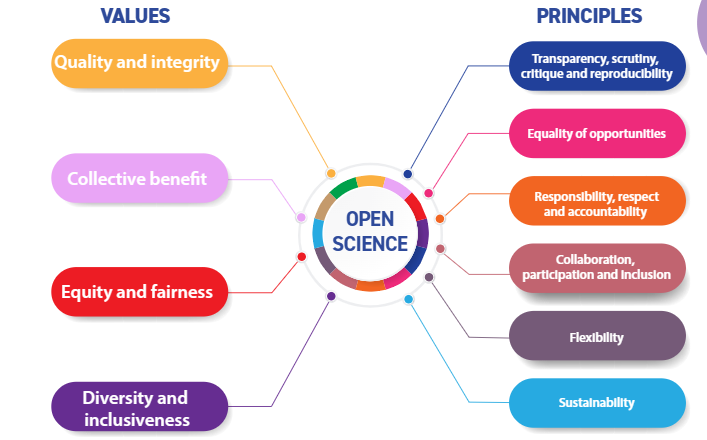
\includegraphics[width=2.08333in,height=\textheight]{capitulos/cap1/images/Captura de pantalla 2024-05-11 020540.png}

}

\caption{Caption}

\end{figure}

\bookmarksetup{startatroot}

\hypertarget{references}{%
\chapter*{References}\label{references}}
\addcontentsline{toc}{chapter}{References}

\markboth{References}{References}

\hypertarget{refs}{}
\begin{CSLReferences}{0}{0}
\end{CSLReferences}

\bookmarksetup{startatroot}

\hypertarget{taller}{%
\chapter{Taller}\label{taller}}

\textbf{Taller de arranque del grupo de trabajo para unificar
metodologías y determinar las variables a analizar}

Lugar: \href{https://maps.app.goo.gl/hCVkgx3S4XdrRimm7}{Edificio 17 del
Instituto de Ingeniería CEMIE-Oceano}, ciudad de México / en línea

\textbf{Objetivo general:}

Presentar la visión integral del proyecto, su origen, fundamentos
teórico-metodológico y principios de ciencia abierta, para unificar
criterios técnicos entre el grupo central de trabajo e identificar en
conjunto las variables potenciales para los ejercicios de modelación.

\textbf{Objetivos particulares:}

1.~~~~~~~~~~~~ Presentar el proyecto, sus etapas, los productos
comprometidos y tiempos estimados.

2.~~~~~~~~~~~~ Presentar las bases teórico-metodológicas del proyecto
(redes bayesianas), así como los fundamentos de ciencia abierta (FAIR).

3.~~~~~~~~~~~~ Identificar posibles variables a utilizar en el modelaje
del proyecto, así como las fuentes de datos e información relevante en
dos escalas (para el nivel nacional y un caso de estudio potencial a
detalle en la Península de Yucatán).

\textbf{Descripción de las actividades}

Los talleres realizados el 29 y 31 de mayo contaron con la participación
de 14 personas que conforman el grupo núcleo de trabajo del proyecto
(ocho mujeres y seis hombres, tres participando en línea), provenientes
del Instituto de Ingeniería de la UNAM, el Instituto de Ecología A. C. y
la UAM -- Xochimilco. Las listas de participantes se encuentran en este
\href{Taller/Anexo\%201\%20Lista\%20de\%20participantes.pdf}{Archivo}.

El taller se realizó con un enfoque participativo, para lo cual, se
preparó un
\href{https://miro.com/welcomeonboard/ckhlZ3lXY1djM0FXd3ZIZmlpV3FUVXFONGJsUFJ0NGFIaWw0eGdHOHBDalhDdFk1Zjg1MUVOZTNMUmZaNDhPVHwzMDc0NDU3MzUyMDM4MTIwMjcwfDI=?share_link_id=865983900620}{pizarrón
digital} (plataforma Miro) y las presentaciones depositadas en el
\href{https://sw-costas-arenosas.netlify.app/presentaciones\#category=presentaci\%C3\%B3n}{blog
de trabajo para el proyecto}. El instrumento de planeación del taller
(carta descriptiva) con la propuesta de actividades detalladas se
encuentra en el anexo 2.

A continuación, se presentan la descripción del desarrollo de las
actividades durante los tres días de trabajo.

\textbf{Día 1.}

\textbf{1.~~~ Bienvenida y presentación}

Al inicio del taller, el Dr.~Octavio Pérez Maqueo dio una breve
bienvenida al taller e informó que cada día se iba a pasar una lista de
asistencia; además, se le pidió a cada persona señalar si brindaban su
consentimiento libre e informado para el uso de imagen e información
considerando la siguiente leyenda: \emph{``Al marcar esta celda, usted
da el consentimiento para que el proyecto `Estimación de la integridad
ecosistémica de las costas arenosas mexicanas a través de técnicas de
aprendizaje de máquina (CF-2023-G-1497)' haga uso de materiales
(fotos/videos) con su imagen, así como de la información derivada de los
días de taller. Ninguna información privada o sensible será utilizada ni
compartida fuera del marco del proyecto. Muchas gracias.''} (Ver listas
en el anexo 1)

Posteriormente a la información de la lista y consentimiento, se invitó
a cada participante a presentarse brevemente con su nombre e
institución.

\textbf{2.~~~~~ Presentación del contexto y origen del proyecto}

El Dr.~Pérez Maqueo desarrolló una presentación en torno a la pregunta
¿por qué creemos que es necesario un proyecto como este? Para ello, la
exposición contó con los siguientes componentes:

Visión integral

o~~~~~~ Caso particular de las costas

o~~~~~~ Desarrollo de habilidades

¿Cómo sugerimos hacerlo?

o~~~~~~ Co-construcción

o~~~~~~ Ciencia Abierta y principios FAIR

o~~~~~~ Análisis con base en propuesta del SEEA EA

o~~~~~~ Flujos de trabajo (pipelines)

En esta primera presentación se destacaron algunos argumentos de la
necesidad que dio origen al proyecto:

o~~ Fortalecer iniciativas nacionales e internacionales que vemos como
una alternativa viable hacia la sustentabilidad.

o~~ Desarrollar metodologías que nos permitan a nosotros u otras
personas rehacer mañana el análisis que hicimos hoy.

o~~ Aprender sobre nuevas formas de análisis dada la capacidad de datos
y cómputo actuales.

o~~ Analizar a los socioecosistemas de manera integral incorporando las
dependencias espaciales que caracteriza a estos sistemas.

o~~ Implementar los resultados del proyecto en la toma de decisiones.

Las presentaciones están disponibles en el blog donde se subirán los
materiales del proyecto:~

\url{https://sw-costas-arenosas.netlify.app/presentaciones\#category=presentaci\%C3\%B3n}

\textbf{3.~~~~~ Descripción del proyecto y marco teórico}

En la segunda parte de la mañana del día 1, se expusieron las
generalidades del proyecto, el marco conceptual, los compromisos
establecidos para las tres etapas del proyecto, presupuesto, avances y
tiempos estimados.

El objetivo principal del proyecto es ``integrar indicadores bióticos y
abióticos en un índice de integridad ecosistémica, a través de un modelo
causal bajo una aproximación de Inteligencia Artificial Interpretable
(IAI)'':

o~ Nacional

o~ Incorporar la complejidad asociada a ecosistemas costeros

o~ Aprendizaje Automático Interpretable (redes bayesianas)

El resultado principal es proponer una metodología para analizar la
integridad ecosistémica de las costas arenosas de México, con el fin de
incorporarla a las cuentas nacionales de ecosistemas y promover su uso
en distintos instrumentos de política pública.

La entrega de la primera etapa del proyecto es el día 27 de junio de
2024, por lo que dentro de los acuerdos se establecieron las tareas y
responsables para cumplir plenamente con los compromisos (ver tabla de
acuerdos, anexo 3).

Posteriormente, el Dr.~Miguel Equihua brindó un panorama de los
fundamentos teóricos en los que se sustenta el proyecto, principalmente
explicando el proceso de análisis de interdependencias condicionadas a
partir de las redes bayesianas (directed acyclic graph- DAG) (ver
\href{https://sw-costas-arenosas.netlify.app/presentaciones\#category=presentaci\%C3\%B3n}{blog}):

En la presentación se destacó la importancia de hacer la ciencia
reproducible, lo que es un DAG, su anatomía, la terminología básica
(noto, arista, variable explicativa, respuesta, ancestros,
descendientes), las reglas de independencia condicional y la separación
condicional. Después del planteamiento teórico, se explicó cómo se busca
construir el DAG de integridad costera. Finalmente se presentó el
fundamento de la ciencia abierta y los principios FAIR.

De esta manera, las/os participantes reconocieron las bases del proyecto
y su propuesta de desarrollo. Al terminar la exposición hubo un breve
espacio para algunas dudas o inquietudes, incluyendo a las personas que
atendieron en línea.

\textbf{4.~~~~~ Presentación de la estrategia metodológica}

La siguiente presentación buscó que el grupo cuente con la información
base de la estrategia metodológica del taller, la cual sirvió también
para realizar el ejercicio planeado para el día 2 de trabajo, en el cual
se identificaron las variables y fuentes de información. La presentación
contó con los siguientes elementos:

o~~~~~~ De lo conceptual a lo analítico (de Miro a Nética)

o~~~~~~ Enfoque causal y probabilístico

o~~~~~~ Documentación y gestión de datos

A lo largo del día se plantearon diversas inquietudes, por ejemplo:

o~~~~~~ Definir las fronteras del área de estudio.

o~~~~~~ Definir si el grupo estaba en posibilidades de un estudio de
caso a profundidad en la Península d Yucatán.

o~~~~~~ Considerar si se considerará información de la cuenca a nivel
superficial y/o a los acuíferos.

o~~~~~~ Definir la temporalidad, qué años y si se toman las dos
temporadas para las costas.

o·~~~~~~ Necesidad de llegar a las resoluciones espaciales para la
información a nivel nacional y para un estudio de caso.

Además, se enlistó la información que podría ser relevante y algunas
fuentes de datos que debían retomarse:

o~ Las imágenes que se usaron para el inventario de humedales, que tiene
imágenes desde el 75 u 83 y del 2005-2006. Consultar a CONABIO.

o~ Las imágenes de los vuelos que tiene INEGI y/o SEMARNAT.

o~ Biblioteca de imágenes de ICA, donde incluso se cuenta con vuelos de
los años sesenta (aerofotos).

o~ Acervo de la compañía mexicana de aerofoto, que se había depositado
en el Instituto de Geografía-UNAM, sin embargo, como no estaban cuidados
los rollos, ICA se los llevo. Los tiene la Fundación ICA.

o~ Las fotografías aéreas más antiguas que tomaron los EE. UU., las
cuales están escaneadas. El equipo de Rodolfo Silva tiene acceso a esta
información. Una parte ya está digitalizada, pero no toda está
organizada, hay mucho trabajo pendiente.

o~ Información de la CFE.

o~ Las cartas geológico-mineras de todo el país. Los tiene el servicio
geológico mexicano

El equipo facilitador tomó notas cada día de trabajo de estos puntos
para llegar a definiciones en una tabla de acuerdos al final del taller
(ver anexo 3).

Al final del día 1, se dio un espacio en plenaria de cierre de la
jornada de trabajo y se propusieron los mecanismos de interacción para
el día 2.

\textbf{Día 2}

\textbf{5.~~~~~ Presentación del tema gestión de datos y presentación de
variables}

Al inicio del día 2, se continuó con el tema de gestión de datos y se
presentaron las temáticas de variables existentes y nuevas variables,
así como las sugerencias para documentar y gestionar datos en el marco
del proyecto.

Posteriormente se brindó un ejemplo de variables y sus interacciones. De
esta manera, el grupo conoció la metodología específica para definir
variables e interacciones.

\textbf{6.~~~~~ Ejercicio participativo de identificación de variables}

a)~~~~~ Mecánica del ejercicio:

Una vez que se introdujo al grupo de trabajo a la metodología de
identificación de variables, se realizó un ejercicio donde el grupo
participó a través de notas digitales tipo post-it en un pizarrón
digital en la plataforma Miro (ver Fig. 1). Para esto, el equipo
facilitador había preparado previamente el pizarrón de trabajo, se
propusieron variables que ya se habían identificado, además de presentar
el ejemplo de un caso que se desarrolló en un proyecto previo.

4.~~~~~~~~~~~~ Definir los parámetros técnicos para el intercambio de
información entre el equipo de trabajo (resolución, formato, metadatos,
etc.).

\textbf{Resultados generados:}

1.~~~~~~~~~~~~~~~~~~~~ Mural digital con la lista de variables
potenciales identificada por el grupo de trabajo, la cual incluye fuente
de datos, la escala de información y la persona que propuso la variable
y que podría gestionar el acceso a la información.

2.~~~~~~~~~~~~~~~~~~~~ Lista de fuentes de información adicionales que
puedan servir como insumo para el modelaje.

3.~~~~~~~~~~~~~~~~~~~~ Tabla de acuerdos con tareas y responsables para
la siguiente fase del proyecto.

\hypertarget{bibliography-references.bib}{%
\section{bibliography:
references.bib}\label{bibliography-references.bib}}

(\textbf{Harper2022?})



\end{document}
